% !TEX root = supp.tex
% Supplementary material body. Input by supp.tex (standalone PDF; the main PDF no longer carries it).
\renewcommand{\thefigure}{S\arabic{figure}}
\renewcommand{\thetable}{S\arabic{table}}
\paragraph{Reproducibility.}
Every number in the paper maps to a CSV and a configuration file in the released log; the benchmark is 700 lines of Python with no training, and all its model runs fit on one 16 GB GPU in about eight hours. The support head trains in about 25 minutes on one GPU from the released configuration; its runs are logged under the P3 run ids.

\begin{figure}[h]
\centering
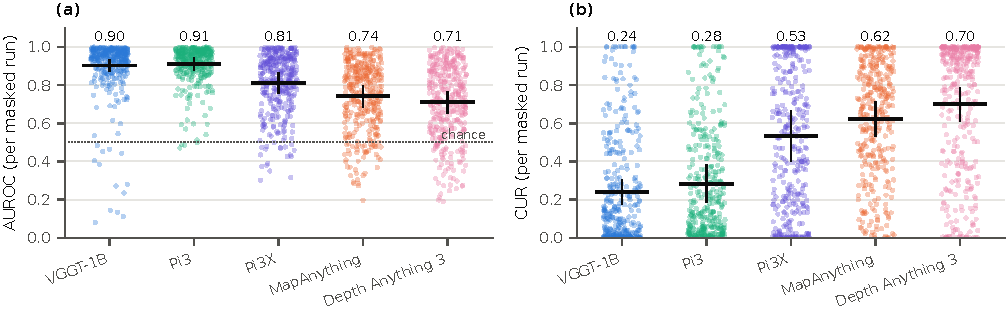
\includegraphics[width=0.95\textwidth]{fig3_metrics}
\caption{\textbf{Per-run spread on DTU.} \auroc{} and \cur{} for every (scan, seed, radius) run under blur and noise fills, with pooled means and intervals. The spread across scans is wide for every model; the intervals in the main tables come from resampling scans.}
\label{fig:metrics}
\end{figure}
\begin{figure}[h]
\centering
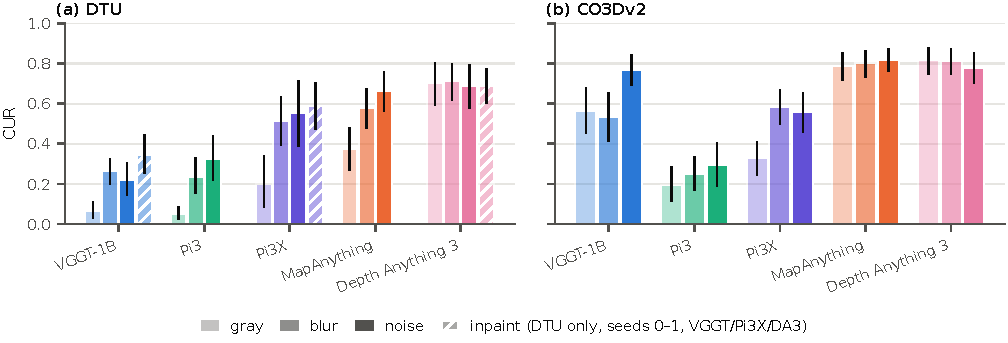
\includegraphics[width=0.95\textwidth]{fig5_fills}
\caption{\textbf{Fill ablation.} \cur{} per model and fill on DTU and CO3Dv2 (five seeds) and for the inpainted fill on DTU (two seeds, three models). A visible gray patch gives the lowest leakage; natural-statistics and inpainted fills give more.}
\label{fig:fills}
\end{figure}
\begin{figure}[h]
\centering
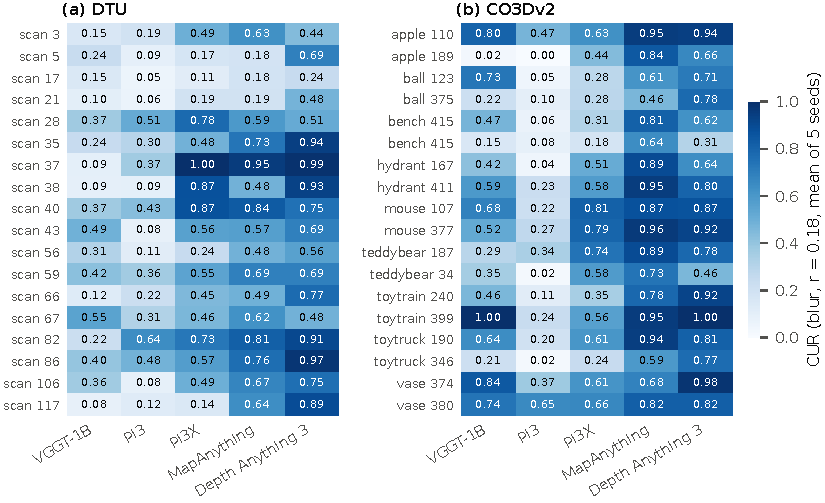
\includegraphics[width=0.95\textwidth]{fig7_perscene}
\caption{\textbf{Per-scene \cur{}} (blur fill, radius 0.18, mean over seeds) for every model on DTU scans and CO3Dv2 scenes. Rows are scenes, columns are models.}
\label{fig:perscene}
\end{figure}

\paragraph{Correctness guards.}
Before any model is scored we check that ground-truth depth reprojects consistently between view pairs and that unsupported points of view $i$, where visible in view $j$, land inside view $j$'s hidden mask. DTU: reprojection agreement 0.80 to 0.82 at a 1\% depth tolerance, U-transfer 0.96 to 0.99. CO3Dv2 (cameras converted from PyTorch3D and checked against the official point cloud): with an occlusion-aware 3\% tolerance, agreement 0.92 to 1.00 and U-transfer 0.90 to 0.98 on 17 of 18 scenes; the eighteenth scores 0.80, is kept, and removing it changes nothing (Section~4 of the paper). ETH3D: agreement 0.996 to 1.000 on all scenes; nine of twelve pass the U-transfer gate and three are excluded before any model is run.

\paragraph{Pipeline validation.}
On a synthetic DTU-format scene, an oracle that knows what is hidden scores \auroc{} 1.000 and \cur{} 0.000, and a blind guesser with flat confidence scores \auroc{} 0.500 and \cur{} 0.90 (the 10\% of supported pixels dropped by $\tau$ is the expected floor). These numbers validate the code, not any model.

\paragraph{Table 1 with intervals.}
The paper's Table 1 shows means; Table~\ref{tab:leak_full} adds 95\% cluster-bootstrap intervals over scenes, \curerr{} and the confidence ratio (median confidence inside the hidden region over its clean value), with the matched split's \auroc$_m$ and \cur$_m$.

\begin{table}[h]
\centering
\caption{\textbf{Native confidence, full numbers.} Blur and noise pooled, 18 scenes $\times$ 5 seeds $\times$ 2 radii; mean [95\% CI]; matched split seeds 0 and 1, radius 0.18. Runs P1-full, P2-full, P2-co3d, P2-co3d-b, P11-matched.}
\label{tab:leak_full}
\footnotesize
\setlength{\tabcolsep}{3pt}
\resizebox{\textwidth}{!}{% generated by scripts/make_tab_leak.py from results/table1_all_models.csv and table3_all_models.csv
\begin{tabular}{l*{2}{cccccc}}
\toprule
model & \multicolumn{6}{c}{DTU, 18 scans} & \multicolumn{6}{c}{CO3Dv2, 18 scenes} \\
 & \auroc$\uparrow$ & \cur$\downarrow$ & \curerr$\downarrow$ & conf ratio & \auroc$_m\uparrow$ & \cur$_m\downarrow$ & \auroc$\uparrow$ & \cur$\downarrow$ & \curerr$\downarrow$ & conf ratio & \auroc$_m\uparrow$ & \cur$_m\downarrow$ \\
\midrule
VGGT-1B & \ci{0.903}{0.873}{0.929} & \ci{0.242}{0.181}{0.304} & 0.000 & 0.22 & 0.551 & 0.802 & \ci{0.681}{0.632}{0.729} & \ci{0.651}{0.566}{0.734} & 0.031 & 0.70 & 0.486 & 0.852 \\
Pi3 & \ci{0.912}{0.881}{0.940} & \ci{0.281}{0.189}{0.379} & 0.002 & 0.34 & 0.495 & 0.828 & \ci{0.891}{0.845}{0.930} & \ci{0.272}{0.190}{0.360} & 0.002 & 0.43 & 0.494 & 0.808 \\
Pi3X & \ci{0.813}{0.762}{0.860} & \ci{0.532}{0.403}{0.663} & 0.003 & 0.91 & 0.474 & 0.870 & \ci{0.732}{0.680}{0.779} & \ci{0.570}{0.500}{0.641} & 0.001 & 0.87 & 0.500 & 0.806 \\
MapAnything & \ci{0.743}{0.687}{0.795} & \ci{0.622}{0.534}{0.707} & 0.286 & 0.69 & 0.515 & 0.837 & \ci{0.576}{0.521}{0.632} & \ci{0.810}{0.756}{0.863} & 0.007 & 0.68 & 0.493 & 0.836 \\
Depth Anything 3 & \ci{0.711}{0.653}{0.763} & \ci{0.701}{0.614}{0.784} & 0.002 & 0.83 & 0.425 & 0.854 & \ci{0.620}{0.567}{0.670} & \ci{0.797}{0.728}{0.861} & 0.000 & 0.88 & 0.482 & 0.839 \\
\bottomrule
\end{tabular}
}
\end{table}

\paragraph{DTU and CO3Dv2, full configuration per fill.}

\begin{table}[h]
\centering
\caption{\textbf{DTU, five models, full configuration.} 18 scans $\times$ 5 mask seeds $\times$ 2 radii $\times$ 3 fills, pooled over radii; mean [95\% cluster-bootstrap CI over scans]. \emph{conf ratio} is the median confidence inside the hidden region divided by its value under clean input. Runs P1-full and P2-full, T4, fp16. The pooled numbers are in Table 1 of the main paper.}
\label{tab:dtu_full}
\footnotesize
\setlength{\tabcolsep}{4pt}
\begin{tabular}{llcccccc}
\toprule
model & fill & \auroc & \cur & \curerr & $\absrel_U$ & $\absrel_U$ ctrl & conf ratio \\
\midrule
VGGT-1B & gray  & \ci{0.973}{0.955}{0.987} & \ci{0.067}{0.031}{0.111} & 0.000 & 0.018 & 0.006 & 0.051 \\
VGGT-1B & blur  & \ci{0.886}{0.843}{0.922} & \ci{0.263}{0.203}{0.324} & 0.000 & 0.011 & 0.006 & 0.241 \\
VGGT-1B & noise & \ci{0.919}{0.892}{0.945} & \ci{0.222}{0.145}{0.304} & 0.000 & 0.014 & 0.006 & 0.192 \\
Pi3 & gray  & \ci{0.981}{0.972}{0.988} & \ci{0.053}{0.025}{0.085} & 0.001 & 0.020 & 0.014 & 0.057 \\
Pi3 & blur  & \ci{0.923}{0.895}{0.947} & \ci{0.236}{0.156}{0.326} & 0.001 & 0.018 & 0.014 & 0.261 \\
Pi3 & noise & \ci{0.902}{0.865}{0.934} & \ci{0.325}{0.219}{0.438} & 0.002 & 0.020 & 0.014 & 0.411 \\
Pi3X & gray  & \ci{0.940}{0.902}{0.971} & \ci{0.202}{0.085}{0.337} & 0.002 & 0.022 & 0.017 & 0.335 \\
Pi3X & blur  & \ci{0.826}{0.782}{0.865} & \ci{0.512}{0.397}{0.630} & 0.002 & 0.020 & 0.017 & 0.739 \\
Pi3X & noise & \ci{0.801}{0.734}{0.864} & \ci{0.551}{0.390}{0.711} & 0.004 & 0.022 & 0.017 & 1.091 \\
MapAnything & gray  & \ci{0.861}{0.812}{0.905} & \ci{0.374}{0.272}{0.480} & \ci{0.195}{0.125}{0.269} & 0.222 & 0.111 & 0.650 \\
MapAnything & blur  & \ci{0.773}{0.720}{0.825} & \ci{0.580}{0.482}{0.672} & \ci{0.277}{0.197}{0.361} & 0.135 & 0.111 & 0.677 \\
MapAnything & noise & \ci{0.712}{0.645}{0.773} & \ci{0.664}{0.566}{0.758} & \ci{0.295}{0.211}{0.390} & 0.129 & 0.111 & 0.709 \\
Depth Anything 3 & gray  & \ci{0.723}{0.664}{0.780} & \ci{0.703}{0.596}{0.804} & 0.003 & 0.017 & 0.013 & 0.804 \\
Depth Anything 3 & blur  & \ci{0.682}{0.611}{0.744} & \ci{0.711}{0.619}{0.796} & 0.003 & 0.016 & 0.013 & 0.800 \\
Depth Anything 3 & noise & \ci{0.740}{0.686}{0.793} & \ci{0.690}{0.578}{0.793} & 0.001 & 0.017 & 0.013 & 0.855 \\
\bottomrule
\end{tabular}
\end{table}

\begin{table}[h]
\centering
\caption{\textbf{CO3Dv2, five models, full configuration.} 18 scenes $\times$ 5 seeds $\times$ 2 radii $\times$ 3 fills, pooled over radii; mean [95\% CI over scenes]. Runs P2-co3d and P2-co3d-b. The pooled numbers are quoted in Section 5.3 of the main paper.}
\label{tab:co3d}
\footnotesize
\setlength{\tabcolsep}{3pt}
\resizebox{\textwidth}{!}{\begin{tabular}{llccccccc}
\toprule
model & fill & \auroc & \cur & \curerr & $\absrel_S$ & $\absrel_U$ & $\absrel_U$ ctrl & conf ratio \\
\midrule
VGGT-1B & gray  & \ci{0.747}{0.692}{0.802} & \ci{0.565}{0.453}{0.677} & 0.029 & 0.029 & 0.031 & 0.027 & 0.634 \\
VGGT-1B & blur  & \ci{0.772}{0.717}{0.825} & \ci{0.534}{0.416}{0.652} & 0.034 & 0.029 & 0.031 & 0.027 & 0.603 \\
VGGT-1B & noise & \ci{0.590}{0.517}{0.656} & \ci{0.767}{0.693}{0.839} & 0.029 & 0.029 & 0.029 & 0.027 & 0.805 \\
Pi3 & gray  & \ci{0.930}{0.894}{0.958} & \ci{0.196}{0.118}{0.283} & 0.002 & 0.015 & 0.016 & 0.013 & 0.351 \\
Pi3 & blur  & \ci{0.903}{0.860}{0.939} & \ci{0.251}{0.170}{0.334} & 0.002 & 0.015 & 0.016 & 0.013 & 0.389 \\
Pi3 & noise & \ci{0.880}{0.813}{0.929} & \ci{0.293}{0.193}{0.405} & 0.002 & 0.015 & 0.015 & 0.013 & 0.472 \\
Pi3X & gray  & \ci{0.863}{0.825}{0.899} & \ci{0.329}{0.248}{0.408} & 0.001 & 0.017 & 0.022 & 0.014 & 0.749 \\
Pi3X & blur  & \ci{0.720}{0.661}{0.777} & \ci{0.584}{0.500}{0.668} & 0.002 & 0.017 & 0.018 & 0.014 & 0.877 \\
Pi3X & noise & \ci{0.743}{0.680}{0.798} & \ci{0.556}{0.462}{0.650} & 0.001 & 0.017 & 0.019 & 0.014 & 0.867 \\
MapAnything & gray  & \ci{0.609}{0.554}{0.665} & \ci{0.786}{0.721}{0.849} & 0.004 & 0.041 & 0.029 & 0.034 & 0.632 \\
MapAnything & blur  & \ci{0.575}{0.514}{0.637} & \ci{0.801}{0.735}{0.863} & 0.008 & 0.042 & 0.028 & 0.034 & 0.674 \\
MapAnything & noise & \ci{0.578}{0.524}{0.631} & \ci{0.819}{0.765}{0.870} & 0.007 & 0.041 & 0.033 & 0.034 & 0.690 \\
Depth Anything 3 & gray  & \ci{0.619}{0.560}{0.674} & \ci{0.816}{0.751}{0.877} & 0.001 & 0.019 & 0.015 & 0.014 & 0.874 \\
Depth Anything 3 & blur  & \ci{0.622}{0.574}{0.668} & \ci{0.813}{0.748}{0.872} & 0.001 & 0.018 & 0.015 & 0.014 & 0.853 \\
Depth Anything 3 & noise & \ci{0.618}{0.553}{0.679} & \ci{0.780}{0.702}{0.854} & 0.000 & 0.019 & 0.016 & 0.014 & 0.901 \\
\bottomrule
\end{tabular}}
\end{table}

\paragraph{Lab rig versus phone captures, plotted.}

\begin{figure}[h]
\centering
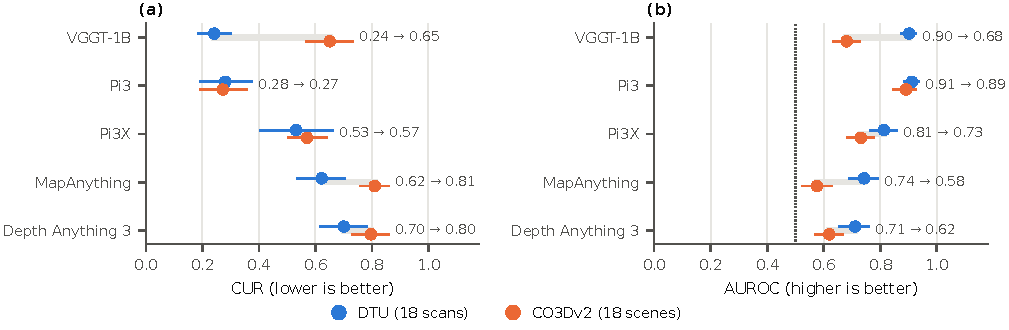
\includegraphics[width=0.8\textwidth]{fig4_dtu_vs_co3d}
\caption{\textbf{Lab rig versus phone captures.} Pooled blur-and-noise \cur{} and \auroc{} per model on DTU and CO3Dv2 with 95\% intervals. Pi3 is the only model whose numbers transfer; VGGT, MapAnything and DA3 leak markedly more on CO3Dv2.}
\label{fig:dtuco3d}
\end{figure}


\paragraph{The benchmark protocol, in a figure.}

\begin{figure}[h]
\centering
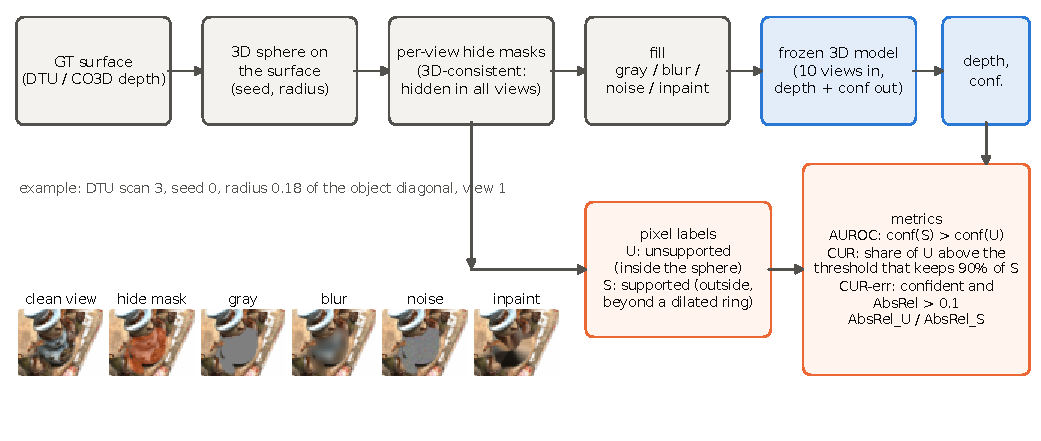
\includegraphics[width=0.8\textwidth]{fig2_pipeline}
\caption{\textbf{The benchmark protocol.} A sphere is placed on the ground-truth surface; every pixel in every view whose ground-truth point falls inside it is hidden, so the hidden region is 3D-consistent. Hidden pixels are filled (gray, blur, noise or inpaint), the model runs on the filled views, and its depth and confidence are scored against the unsupported (U), supported (S) and ring labels. The same pixels are also scored under clean input as a control.}
\label{fig:pipeline}
\end{figure}

\paragraph{The filled patch, in pictures.}

\begin{figure}[h]
\centering
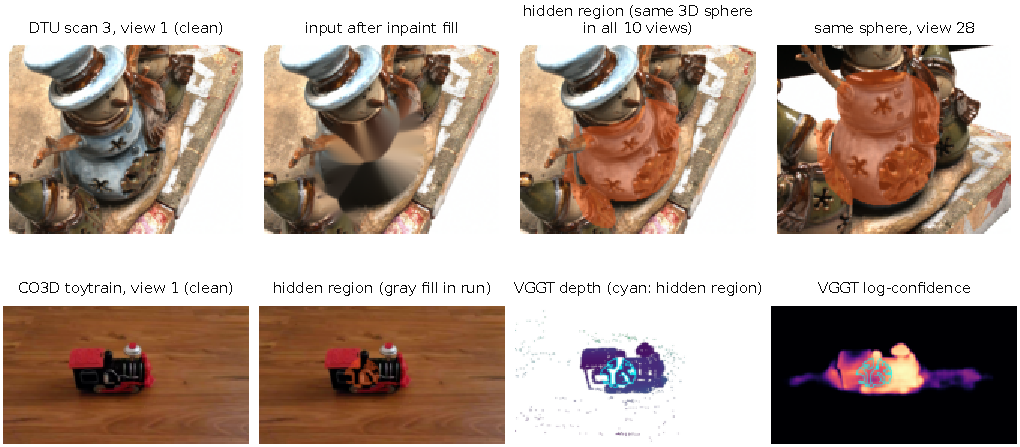
\includegraphics[width=0.7\textwidth]{fig1_teaser}
\caption{\textbf{What a model does with a surface it cannot see.} Top: a DTU scan with one 3D region of the ground-truth surface hidden in all ten input views and inpainted so no seam remains (the inpainted fill of Section~4 of the paper). Bottom: a CO3Dv2 phone capture treated the same way. The top row shows the protocol: the same 3D sphere hides the region in every view, including a view from the other side of the rig. The bottom row shows what the backbone (VGGT) does with it: plausible geometry inside the hidden region, with confidence close to its value outside. The cyan contour marks the unsupported pixels. Model panels are the recorded run outputs.}
\label{fig:teaser}
\end{figure}

\paragraph{Fused point clouds at matched coverage.}
Each backbone's per-view depths are back-projected with its own predicted cameras into one cloud, aligned to the ground-truth frame by a similarity transform fitted on the camera centres, and compared with the ground-truth cloud of the same views at a tolerance of 1\% of the scene's median depth: accuracy is the fraction of predicted points within tolerance of a ground-truth point, completeness the converse. A detector keeps the given fraction of points with the highest score; random dropping and an oracle that drops single-view pixels first are the references. Table~\ref{tab:fuse}: 18 DTU scans and 9 ETH3D scenes, 5 and 10 views, two view sets, run P8-fuse; the rows marked $\times$ are the label-free head multiplied by native confidence. The absolute accuracies on ETH3D are low because the predicted cameras of a building scan align poorly to the laser frame; the comparison between detectors at matched coverage is what the table is for.

\begin{table}[h]
\centering
\caption{\textbf{Fused point cloud at matched coverage}, accuracy / completeness against the laser or MVS cloud.}
\label{tab:fuse}
\footnotesize
\setlength{\tabcolsep}{4pt}
\resizebox{\textwidth}{!}{% generated by scripts/make_tab_vis.py from results/P8-fuse
\begin{tabular}{l*{6}{c}}
\toprule
detector & \multicolumn{3}{c}{DTU, accuracy / completeness} & \multicolumn{3}{c}{ETH3D, accuracy / completeness} \\
coverage & 0.6 & 0.8 & 1.0 & 0.6 & 0.8 & 1.0 \\
\midrule
native confidence & 0.842 / 0.804 & 0.783 / 0.885 & 0.653 / 0.902 & 0.337 / 0.396 & 0.306 / 0.443 & 0.273 / 0.470 \\
reprojection consistency & 0.805 / 0.837 & 0.763 / 0.868 & 0.654 / 0.902 & 0.321 / 0.413 & 0.302 / 0.438 & 0.273 / 0.470 \\
per-image control & 0.766 / 0.735 & 0.698 / 0.835 & 0.653 / 0.902 & 0.293 / 0.369 & 0.281 / 0.428 & 0.273 / 0.470 \\
label-free head & 0.834 / 0.770 & 0.771 / 0.874 & 0.653 / 0.902 & 0.331 / 0.383 & 0.300 / 0.428 & 0.273 / 0.470 \\
random dropping & 0.653 / 0.896 & 0.653 / 0.900 & 0.653 / 0.902 & 0.273 / 0.462 & 0.273 / 0.467 & 0.273 / 0.470 \\
oracle: single-view first & 0.699 / 0.833 & 0.663 / 0.863 & 0.653 / 0.902 & 0.273 / 0.417 & 0.275 / 0.442 & 0.273 / 0.470 \\
label-free head $\times$ native confidence & 0.844 / 0.786 & 0.785 / 0.883 & 0.653 / 0.902 & 0.333 / 0.384 & 0.304 / 0.437 & 0.273 / 0.470 \\
native confidence (Pi3X) & 0.381 / 0.498 & 0.349 / 0.543 & 0.297 / 0.562 & 0.346 / 0.426 & 0.314 / 0.467 & 0.272 / 0.482 \\
reprojection (Pi3X) & 0.353 / 0.485 & 0.350 / 0.535 & 0.297 / 0.559 & 0.301 / 0.412 & 0.297 / 0.439 & 0.273 / 0.481 \\
label-free head (Pi3X) & 0.404 / 0.494 & 0.354 / 0.546 & 0.297 / 0.562 & 0.332 / 0.404 & 0.299 / 0.446 & 0.272 / 0.482 \\
label-free head $\times$ native (Pi3X) & 0.403 / 0.492 & 0.356 / 0.547 & 0.297 / 0.562 & 0.338 / 0.408 & 0.306 / 0.454 & 0.272 / 0.481 \\
oracle (Pi3X) & 0.310 / 0.500 & 0.300 / 0.531 & 0.297 / 0.562 & 0.260 / 0.418 & 0.268 / 0.449 & 0.272 / 0.482 \\
\bottomrule
\end{tabular}
}
\end{table}

\paragraph{Detectors on the filled patches.}
The cheap alternatives and the fill-trained heads of Sections 4 and 6 of the main paper, on the Table 1 rows with blur, radius 0.18 and seed 0. A fuller perturbation baseline (photometric, blur, flip and view-permutation perturbations, $K=8$, least-squares scale alignment, median-absolute-deviation spread; run P3-pv-full) scores \auroc{} 0.52 to 0.60 and \cur{} 0.74 to 0.86 on all five backbones over blur and noise, worse than native confidence everywhere. On 22 further DTU scans (the MVSNet test split, run P3-dtuext, seed 0, radius 0.18) the ranking of Table 1 holds: VGGT \auroc{} 0.908 / \cur{} 0.233, Pi3 0.919 / 0.272, Pi3X 0.850 / 0.539, DA3 0.755 / 0.650, MapAnything 0.697 / 0.693 with \curerr{} 0.287. On the nine ETH3D scenes under the full fill protocol (run P3-eth3d) native confidence leaks more than on DTU, \cur{} 0.61 (Pi3) to 0.79 (VGGT), and the fill-trained head scores 0.981 against its per-image control's 0.987.

\begin{table}[h]
\centering
\caption{\textbf{Detectors on the filled patches, DTU} (18 scans, seed 0, blur, radius 0.18; native and perturbation rows re-run on the detectors' hardware, runs P3-native and P3-pv, so every pair is scored on identical rows). The three learned rows per backbone are the \emph{fill-trained} heads: they find the fill, not the missing support (Section~5 of the paper), which is why the per-image control matches them. The visibility-trained heads are in the main paper.}
\label{tab:detectors}
\footnotesize
\setlength{\tabcolsep}{3pt}
\resizebox{0.7\textwidth}{!}{\begin{tabular}{llccc}
\toprule
backbone & detector & fwd & \auroc & \cur \\
\midrule
VGGT-1B & native confidence & 1 & \ci{0.915}{0.883}{0.943} & \ci{0.255}{0.157}{0.364} \\
VGGT-1B & perturbation var., $K{=}4$ & 4 & \ci{0.666}{0.602}{0.729} & \ci{0.627}{0.521}{0.732} \\
VGGT-1B & reprojection consistency & 1 & \ci{0.488}{0.473}{0.506} & \ci{0.931}{0.903}{0.954} \\
VGGT-1B & fill-trained linear probe & 1 & \ci{1.000}{1.000}{1.000} & \ci{0.000}{0.000}{0.000} \\
VGGT-1B & fill-trained per-image control & 1 & \ci{1.000}{1.000}{1.000} & \ci{0.000}{0.000}{0.000} \\
VGGT-1B & fill-trained support head & 1 & \ci{1.000}{1.000}{1.000} & \ci{0.000}{0.000}{0.000} \\
Pi3X & native confidence & 1 & \ci{0.832}{0.782}{0.879} & \ci{0.502}{0.362}{0.642} \\
Pi3X & perturbation var., $K{=}4$ & 4 & \ci{0.550}{0.491}{0.608} & \ci{0.824}{0.754}{0.886} \\
Pi3X & reprojection consistency & 1 & \ci{0.478}{0.435}{0.518} & \ci{0.929}{0.899}{0.955} \\
Pi3X & fill-trained per-image control & 1 & \ci{1.000}{0.999}{1.000} & \ci{0.000}{0.000}{0.001} \\
Pi3X & fill-trained support head & 1 & \ci{0.999}{0.999}{1.000} & \ci{0.001}{0.000}{0.003} \\
\bottomrule
\end{tabular}}
\end{table}

\paragraph{Stress tests.}
Section 5.2 of the main paper summarises this table.

\begin{table}[h]
\centering
\caption{\textbf{Stress tests on DTU.} 18 scans $\times$ 2 mask seeds, radius 0.18, models VGGT, Pi3X, DA3. Reference rows are the matching cells of Table~1 of the paper (blur, 10 spread views, seeds 0 and 1). Last column: paired \cur{} difference against the reference with a sign-flip $p$ over scans. Run P2-stress.}
\label{tab:stress}
\footnotesize
\setlength{\tabcolsep}{4pt}
\begin{tabular}{llccccl}
\toprule
model & test & \auroc & \cur & \curerr & $\absrel_U$ & \cur{} vs ref \\
\midrule
VGGT-1B & reference & \ci{0.902}{0.868}{0.930} & \ci{0.259}{0.175}{0.349} & 0.000 & 0.010 & \\
VGGT-1B & inpaint fill & \ci{0.867}{0.821}{0.907} & \ci{0.347}{0.255}{0.443} & 0.001 & 0.018 & $+0.088$ ($p=0.031$) \\
VGGT-1B & 5 views & 0.902 & \ci{0.269}{0.173}{0.377} & 0.000 & 0.011 & $+0.010$ ($p=0.63$) \\
VGGT-1B & 3 views & 0.899 & \ci{0.259}{0.167}{0.361} & 0.000 & 0.013 & $+0.001$ ($p=0.98$) \\
VGGT-1B & low parallax & 0.911 & \ci{0.214}{0.110}{0.334} & 0.000 & 0.021 & $-0.045$ ($p=0.35$) \\
VGGT-1B & + distractor & 0.905 & \ci{0.257}{0.179}{0.340} & 0.000 & 0.011 & $-0.002$ ($p=0.90$) \\
Pi3X & reference & \ci{0.828}{0.781}{0.870} & \ci{0.521}{0.390}{0.650} & 0.002 & 0.024 & \\
Pi3X & inpaint fill & \ci{0.786}{0.731}{0.836} & \ci{0.589}{0.473}{0.702} & 0.004 & 0.022 & $+0.068$ ($p=0.005$) \\
Pi3X & 5 views & 0.822 & \ci{0.539}{0.411}{0.661} & 0.006 & 0.024 & $+0.018$ ($p=0.44$) \\
Pi3X & 3 views & 0.840 & \ci{0.497}{0.373}{0.618} & 0.032 & 0.051 & $-0.024$ ($p=0.64$) \\
Pi3X & low parallax & 0.812 & \ci{0.523}{0.376}{0.671} & 0.040 & 0.050 & $+0.002$ ($p=0.98$) \\
Pi3X & + distractor & 0.829 & \ci{0.510}{0.368}{0.650} & 0.002 & 0.024 & $-0.011$ ($p=0.66$) \\
DA3 & reference & \ci{0.712}{0.632}{0.783} & \ci{0.679}{0.569}{0.791} & 0.006 & 0.018 & \\
DA3 & inpaint fill & 0.726 & \ci{0.688}{0.605}{0.774} & 0.009 & 0.018 & $+0.008$ ($p=0.87$) \\
DA3 & 5 views & 0.697 & \ci{0.785}{0.703}{0.865} & 0.005 & 0.019 & $+0.106$ ($p=0.008$) \\
DA3 & 3 views & 0.729 & \ci{0.667}{0.560}{0.770} & 0.018 & 0.031 & $-0.012$ ($p=0.81$) \\
DA3 & low parallax & \ci{0.863}{0.785}{0.925} & \ci{0.372}{0.230}{0.520} & 0.008 & 0.029 & $-0.307$ ($p=0.0003$) \\
DA3 & + distractor & \ci{0.660}{0.580}{0.734} & \ci{0.775}{0.680}{0.868} & 0.003 & 0.019 & $+0.096$ ($p=0.0004$) \\
\bottomrule
\end{tabular}
\end{table}


\paragraph{Stress tests, plotted.}

\begin{figure}[h]
\centering
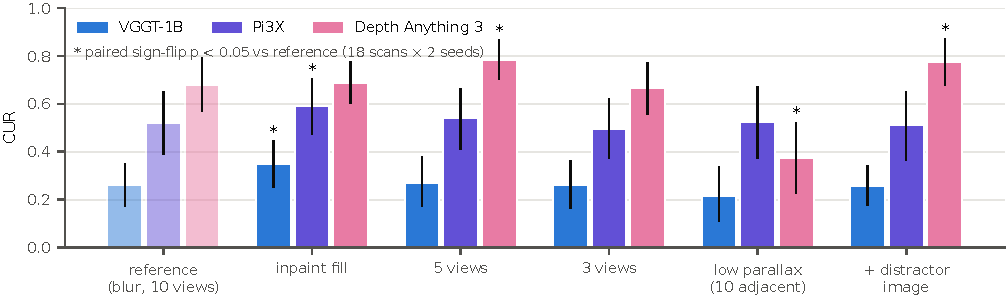
\includegraphics[width=0.8\textwidth]{fig6_stress}
\caption{\textbf{Stress tests.} \cur{} under each stress condition against the reference, with intervals. View count does nothing for VGGT and Pi3X; the inpainted fill raises leakage; DA3 alone reacts to parallax and to a distractor.}
\label{fig:stress}
\end{figure}


\paragraph{Every detector on the true-visibility protocol.}
Table~\ref{tab:vis_supp} lists every detector of the main paper's Table 3 with 95\% cluster-bootstrap intervals over scenes, including the fill-trained heads and the linear probe trained on self-support labels. Per-view-count tables, the per-layer probes and every paired test are in the released statistics file (\texttt{results/P3-stats.md}).

\begin{table}[h]
\centering
\caption{\textbf{True-visibility protocol, every detector}, pooled over scenes and view counts as in the main paper, with 95\% cluster-bootstrap intervals over scenes.}
\label{tab:vis_supp}
\tiny
\setlength{\tabcolsep}{2pt}
\resizebox{\textwidth}{!}{% generated by scripts/make_tab_vis.py from results/P4-vis*, P7-vis-imc, P6-adapt-*, P7-adapt-imc
\begin{tabular}{l*{4}{cc}}
\toprule
detector & \multicolumn{2}{c}{DTU} & \multicolumn{2}{c}{CO3Dv2} & \multicolumn{2}{c}{ETH3D} & \multicolumn{2}{c}{Photot.} \\
 & \auroc$\uparrow$ & \cur$\downarrow$ & \auroc$\uparrow$ & \cur$\downarrow$ & \auroc$\uparrow$ & \cur$\downarrow$ & \auroc$\uparrow$ & \cur$\downarrow$ \\
\midrule
\multicolumn{9}{l}{\emph{VGGT-1B}} \\
native confidence & \ci{0.772}{0.722}{0.823} & \ci{0.530}{0.443}{0.616} & \ci{0.754}{0.712}{0.793} & \ci{0.723}{0.650}{0.796} & \ci{0.715}{0.621}{0.802} & \ci{0.566}{0.430}{0.704} & \ci{0.802}{0.748}{0.850} & \ci{0.451}{0.343}{0.569} \\
reprojection consistency & \ci{0.954}{0.944}{0.963} & \ci{0.082}{0.067}{0.098} & \ci{0.793}{0.746}{0.839} & \ci{0.693}{0.517}{0.860} & \ci{0.975}{0.968}{0.982} & \ci{0.069}{0.034}{0.106} & \ci{0.824}{0.786}{0.869} & \ci{0.340}{0.249}{0.423} \\
distance to image border & \ci{0.701}{0.671}{0.731} & \ci{0.727}{0.700}{0.755} & \ci{0.454}{0.388}{0.520} & \ci{0.897}{0.834}{0.946} & \ci{0.725}{0.669}{0.780} & \ci{0.632}{0.534}{0.728} & \ci{0.730}{0.695}{0.765} & \ci{0.649}{0.606}{0.689} \\
depth edges & \ci{0.549}{0.519}{0.576} & \ci{0.831}{0.806}{0.855} & \ci{0.422}{0.373}{0.473} & \ci{0.943}{0.923}{0.962} & \ci{0.598}{0.503}{0.699} & \ci{0.762}{0.638}{0.857} & \ci{0.674}{0.594}{0.748} & \ci{0.619}{0.527}{0.714} \\
fill-trained head & \ci{0.609}{0.575}{0.646} & \ci{0.765}{0.728}{0.798} & \ci{0.451}{0.379}{0.522} & \ci{0.916}{0.880}{0.948} & \ci{0.686}{0.615}{0.760} & \ci{0.657}{0.551}{0.758} & \ci{0.704}{0.647}{0.759} & \ci{0.673}{0.594}{0.749} \\
fill-trained per-image control & \ci{0.744}{0.705}{0.779} & \ci{0.640}{0.586}{0.697} & \ci{0.356}{0.306}{0.410} & \ci{0.957}{0.943}{0.969} & \ci{0.619}{0.542}{0.698} & \ci{0.736}{0.641}{0.820} & \ci{0.622}{0.562}{0.686} & \ci{0.760}{0.706}{0.805} \\
per-image control (GT labels) & \ci{0.878}{0.845}{0.907} & \ci{0.340}{0.289}{0.394} & \ci{0.462}{0.392}{0.540} & \ci{0.878}{0.814}{0.933} & \ci{0.712}{0.649}{0.767} & \ci{0.666}{0.608}{0.731} & \ci{0.787}{0.732}{0.837} & \ci{0.530}{0.448}{0.603} \\
linear probe (GT labels) & \ci{0.989}{0.985}{0.992} & \ci{0.024}{0.015}{0.035} & \ci{0.913}{0.883}{0.942} & \ci{0.250}{0.165}{0.337} & \ci{0.966}{0.959}{0.975} & \ci{0.095}{0.068}{0.122} & \ci{0.894}{0.843}{0.936} & \ci{0.265}{0.158}{0.392} \\
support head, GT visibility labels & \ci{0.993}{0.990}{0.995} & \ci{0.015}{0.008}{0.024} & \ci{0.927}{0.903}{0.951} & \ci{0.211}{0.138}{0.287} & \ci{0.980}{0.972}{0.986} & \ci{0.055}{0.035}{0.076} & \ci{0.908}{0.863}{0.947} & \ci{0.258}{0.146}{0.391} \\
per-image control (self labels) & \ci{0.885}{0.851}{0.912} & \ci{0.325}{0.272}{0.383} & \ci{0.460}{0.394}{0.532} & \ci{0.892}{0.833}{0.937} & \ci{0.626}{0.538}{0.711} & \ci{0.750}{0.665}{0.830} & \ci{0.729}{0.656}{0.805} & \ci{0.681}{0.535}{0.810} \\
linear probe (self labels) & \ci{0.988}{0.984}{0.992} & \ci{0.022}{0.014}{0.032} & \ci{0.898}{0.861}{0.934} & \ci{0.296}{0.191}{0.402} & \ci{0.967}{0.958}{0.976} & \ci{0.084}{0.058}{0.107} & \ci{0.924}{0.903}{0.948} & \ci{0.187}{0.127}{0.243} \\
\textbf{support head, label-free} & \ci{0.992}{0.989}{0.995} & \ci{0.017}{0.010}{0.025} & \ci{0.931}{0.907}{0.953} & \ci{0.199}{0.134}{0.266} & \ci{0.980}{0.972}{0.986} & \ci{0.051}{0.033}{0.069} & \ci{0.930}{0.908}{0.954} & \ci{0.191}{0.125}{0.253} \\
label-free head, adapted on the target domain & -- & -- & \ci{0.841}{0.785}{0.891} & \ci{0.474}{0.338}{0.610} & -- & -- & \ci{0.926}{0.899}{0.952} & \ci{0.203}{0.132}{0.275} \\
support head (GT labels) $\times$ native confidence & \ci{0.986}{0.980}{0.990} & \ci{0.031}{0.018}{0.047} & \ci{0.920}{0.891}{0.947} & \ci{0.236}{0.149}{0.338} & \ci{0.954}{0.935}{0.972} & \ci{0.131}{0.071}{0.199} & \ci{0.931}{0.912}{0.952} & \ci{0.177}{0.115}{0.237} \\
label-free head $\times$ native confidence & \ci{0.980}{0.973}{0.986} & \ci{0.048}{0.030}{0.069} & \ci{0.920}{0.890}{0.948} & \ci{0.225}{0.144}{0.314} & \ci{0.943}{0.920}{0.965} & \ci{0.150}{0.086}{0.224} & \ci{0.930}{0.912}{0.951} & \ci{0.179}{0.118}{0.238} \\
\multicolumn{9}{l}{\emph{Pi3X}} \\
native confidence & \ci{0.820}{0.793}{0.845} & \ci{0.493}{0.435}{0.553} & \ci{0.697}{0.649}{0.740} & \ci{0.846}{0.803}{0.888} & \ci{0.887}{0.856}{0.918} & \ci{0.304}{0.213}{0.389} & \ci{0.839}{0.808}{0.867} & \ci{0.450}{0.365}{0.549} \\
reprojection consistency & \ci{0.914}{0.900}{0.929} & \ci{0.164}{0.120}{0.213} & \ci{0.885}{0.859}{0.909} & \ci{0.224}{0.164}{0.293} & \ci{0.977}{0.965}{0.986} & \ci{0.054}{0.024}{0.092} & \ci{0.814}{0.775}{0.857} & \ci{0.361}{0.287}{0.431} \\
distance to image border & \ci{0.701}{0.671}{0.731} & \ci{0.727}{0.700}{0.755} & \ci{0.454}{0.388}{0.520} & \ci{0.897}{0.834}{0.946} & \ci{0.725}{0.669}{0.780} & \ci{0.632}{0.534}{0.728} & \ci{0.730}{0.695}{0.765} & \ci{0.649}{0.606}{0.689} \\
depth edges & \ci{0.545}{0.516}{0.573} & \ci{0.835}{0.812}{0.858} & \ci{0.424}{0.377}{0.474} & \ci{0.951}{0.933}{0.967} & \ci{0.596}{0.498}{0.703} & \ci{0.761}{0.640}{0.854} & \ci{0.638}{0.570}{0.700} & \ci{0.699}{0.640}{0.762} \\
fill-trained head & \ci{0.713}{0.679}{0.745} & \ci{0.650}{0.596}{0.706} & \ci{0.433}{0.378}{0.491} & \ci{0.909}{0.864}{0.942} & \ci{0.647}{0.573}{0.703} & \ci{0.695}{0.643}{0.751} & \ci{0.823}{0.784}{0.863} & \ci{0.454}{0.370}{0.536} \\
fill-trained per-image control & \ci{0.718}{0.681}{0.751} & \ci{0.667}{0.622}{0.715} & \ci{0.391}{0.338}{0.445} & \ci{0.959}{0.948}{0.969} & \ci{0.644}{0.595}{0.695} & \ci{0.719}{0.625}{0.800} & \ci{0.681}{0.631}{0.730} & \ci{0.720}{0.657}{0.781} \\
per-image control (GT labels) & \ci{0.863}{0.831}{0.891} & \ci{0.375}{0.326}{0.425} & \ci{0.428}{0.359}{0.507} & \ci{0.889}{0.823}{0.941} & \ci{0.694}{0.640}{0.749} & \ci{0.685}{0.614}{0.745} & \ci{0.775}{0.722}{0.825} & \ci{0.577}{0.499}{0.651} \\
linear probe (GT labels) & \ci{0.985}{0.979}{0.989} & \ci{0.034}{0.021}{0.049} & \ci{0.931}{0.907}{0.954} & \ci{0.203}{0.133}{0.277} & \ci{0.956}{0.939}{0.970} & \ci{0.123}{0.074}{0.181} & \ci{0.919}{0.894}{0.944} & \ci{0.204}{0.136}{0.271} \\
support head, GT visibility labels & \ci{0.990}{0.986}{0.994} & \ci{0.021}{0.010}{0.035} & \ci{0.930}{0.907}{0.953} & \ci{0.221}{0.138}{0.312} & \ci{0.975}{0.964}{0.984} & \ci{0.072}{0.041}{0.107} & \ci{0.938}{0.919}{0.959} & \ci{0.176}{0.111}{0.240} \\
per-image control (self labels) & \ci{0.871}{0.837}{0.899} & \ci{0.363}{0.309}{0.418} & \ci{0.469}{0.400}{0.546} & \ci{0.877}{0.809}{0.928} & \ci{0.610}{0.531}{0.688} & \ci{0.776}{0.709}{0.831} & \ci{0.719}{0.643}{0.797} & \ci{0.697}{0.566}{0.821} \\
linear probe (self labels) & \ci{0.983}{0.977}{0.988} & \ci{0.036}{0.023}{0.051} & \ci{0.931}{0.903}{0.957} & \ci{0.192}{0.121}{0.269} & \ci{0.939}{0.918}{0.956} & \ci{0.171}{0.114}{0.241} & \ci{0.919}{0.894}{0.945} & \ci{0.200}{0.133}{0.264} \\
\textbf{support head, label-free} & \ci{0.988}{0.983}{0.993} & \ci{0.025}{0.013}{0.040} & \ci{0.939}{0.916}{0.960} & \ci{0.190}{0.118}{0.265} & \ci{0.963}{0.946}{0.976} & \ci{0.103}{0.061}{0.158} & \ci{0.940}{0.920}{0.960} & \ci{0.166}{0.105}{0.226} \\
label-free head, adapted on the target domain & -- & -- & \ci{0.964}{0.947}{0.978} & \ci{0.094}{0.054}{0.143} & -- & -- & \ci{0.929}{0.898}{0.958} & \ci{0.198}{0.118}{0.282} \\
support head (GT labels) $\times$ native confidence & \ci{0.988}{0.983}{0.993} & \ci{0.027}{0.014}{0.042} & \ci{0.928}{0.903}{0.952} & \ci{0.230}{0.144}{0.323} & \ci{0.978}{0.967}{0.987} & \ci{0.064}{0.033}{0.099} & \ci{0.935}{0.911}{0.957} & \ci{0.181}{0.109}{0.258} \\
label-free head $\times$ native confidence & \ci{0.986}{0.980}{0.991} & \ci{0.030}{0.017}{0.046} & \ci{0.935}{0.912}{0.958} & \ci{0.200}{0.124}{0.280} & \ci{0.967}{0.949}{0.980} & \ci{0.092}{0.051}{0.146} & \ci{0.934}{0.910}{0.957} & \ci{0.185}{0.113}{0.258} \\
\multicolumn{9}{l}{\emph{Pi3}} \\
native confidence & \ci{0.841}{0.815}{0.864} & \ci{0.489}{0.426}{0.553} & \ci{0.551}{0.503}{0.600} & \ci{0.882}{0.845}{0.917} & \ci{0.814}{0.756}{0.871} & \ci{0.498}{0.371}{0.618} & \ci{0.847}{0.795}{0.892} & \ci{0.447}{0.345}{0.555} \\
reprojection consistency & \ci{0.952}{0.943}{0.960} & \ci{0.089}{0.069}{0.112} & \ci{0.894}{0.871}{0.915} & \ci{0.205}{0.153}{0.261} & \ci{0.976}{0.965}{0.985} & \ci{0.039}{0.023}{0.058} & \ci{0.817}{0.775}{0.864} & \ci{0.345}{0.250}{0.432} \\
distance to image border & \ci{0.701}{0.671}{0.731} & \ci{0.727}{0.700}{0.755} & \ci{0.454}{0.388}{0.520} & \ci{0.897}{0.834}{0.946} & \ci{0.725}{0.669}{0.780} & \ci{0.632}{0.534}{0.728} & \ci{0.730}{0.695}{0.765} & \ci{0.649}{0.606}{0.689} \\
depth edges & \ci{0.546}{0.518}{0.574} & \ci{0.839}{0.816}{0.862} & \ci{0.424}{0.377}{0.472} & \ci{0.950}{0.932}{0.967} & \ci{0.597}{0.499}{0.704} & \ci{0.764}{0.637}{0.858} & \ci{0.652}{0.583}{0.718} & \ci{0.670}{0.598}{0.745} \\
per-image control (GT labels) & \ci{0.878}{0.846}{0.906} & \ci{0.345}{0.291}{0.402} & \ci{0.464}{0.393}{0.544} & \ci{0.880}{0.815}{0.935} & \ci{0.717}{0.651}{0.774} & \ci{0.661}{0.601}{0.729} & \ci{0.796}{0.744}{0.842} & \ci{0.510}{0.431}{0.583} \\
linear probe (GT labels) & \ci{0.985}{0.980}{0.990} & \ci{0.032}{0.019}{0.046} & \ci{0.943}{0.922}{0.962} & \ci{0.175}{0.109}{0.245} & \ci{0.938}{0.905}{0.965} & \ci{0.165}{0.091}{0.249} & \ci{0.914}{0.882}{0.944} & \ci{0.218}{0.143}{0.290} \\
support head, GT visibility labels & \ci{0.992}{0.988}{0.995} & \ci{0.016}{0.008}{0.026} & \ci{0.934}{0.914}{0.954} & \ci{0.203}{0.135}{0.273} & \ci{0.953}{0.926}{0.974} & \ci{0.135}{0.068}{0.214} & \ci{0.932}{0.911}{0.954} & \ci{0.201}{0.131}{0.272} \\
per-image control (self labels) & \ci{0.888}{0.856}{0.914} & \ci{0.320}{0.268}{0.381} & \ci{0.471}{0.402}{0.548} & \ci{0.895}{0.834}{0.942} & \ci{0.654}{0.579}{0.725} & \ci{0.750}{0.668}{0.822} & \ci{0.724}{0.645}{0.804} & \ci{0.683}{0.533}{0.820} \\
linear probe (self labels) & \ci{0.983}{0.977}{0.989} & \ci{0.031}{0.018}{0.046} & \ci{0.926}{0.897}{0.953} & \ci{0.235}{0.139}{0.335} & \ci{0.917}{0.885}{0.944} & \ci{0.225}{0.151}{0.308} & \ci{0.915}{0.882}{0.945} & \ci{0.209}{0.140}{0.275} \\
\textbf{support head, label-free} & \ci{0.989}{0.984}{0.994} & \ci{0.021}{0.011}{0.034} & \ci{0.930}{0.907}{0.952} & \ci{0.225}{0.145}{0.309} & \ci{0.951}{0.924}{0.971} & \ci{0.139}{0.075}{0.215} & \ci{0.931}{0.908}{0.955} & \ci{0.181}{0.121}{0.238} \\
label-free head $\times$ native confidence & \ci{0.985}{0.979}{0.990} & \ci{0.034}{0.021}{0.048} & \ci{0.915}{0.888}{0.942} & \ci{0.266}{0.172}{0.364} & \ci{0.943}{0.911}{0.966} & \ci{0.151}{0.088}{0.228} & \ci{0.929}{0.907}{0.953} & \ci{0.197}{0.129}{0.257} \\
\multicolumn{9}{l}{\emph{Depth Anything 3}} \\
native confidence & \ci{0.836}{0.815}{0.855} & \ci{0.430}{0.383}{0.481} & \ci{0.683}{0.615}{0.742} & \ci{0.743}{0.655}{0.828} & \ci{0.643}{0.557}{0.744} & \ci{0.635}{0.494}{0.757} & \ci{0.782}{0.707}{0.851} & \ci{0.512}{0.389}{0.636} \\
reprojection consistency & \ci{0.926}{0.912}{0.939} & \ci{0.175}{0.118}{0.241} & \ci{0.836}{0.799}{0.872} & \ci{0.463}{0.335}{0.585} & \ci{0.962}{0.942}{0.977} & \ci{0.109}{0.044}{0.176} & \ci{0.844}{0.804}{0.882} & \ci{0.332}{0.247}{0.419} \\
distance to image border & \ci{0.701}{0.671}{0.731} & \ci{0.727}{0.700}{0.755} & \ci{0.454}{0.388}{0.520} & \ci{0.897}{0.834}{0.946} & \ci{0.725}{0.669}{0.780} & \ci{0.632}{0.534}{0.728} & \ci{0.730}{0.695}{0.765} & \ci{0.649}{0.606}{0.689} \\
depth edges & \ci{0.551}{0.525}{0.576} & \ci{0.844}{0.821}{0.868} & \ci{0.408}{0.356}{0.463} & \ci{0.968}{0.953}{0.981} & \ci{0.592}{0.498}{0.695} & \ci{0.767}{0.643}{0.859} & \ci{0.645}{0.582}{0.707} & \ci{0.717}{0.651}{0.782} \\
per-image control (GT labels) & \ci{0.761}{0.728}{0.794} & \ci{0.586}{0.537}{0.632} & \ci{0.440}{0.373}{0.506} & \ci{0.903}{0.842}{0.947} & \ci{0.746}{0.701}{0.794} & \ci{0.620}{0.535}{0.700} & \ci{0.732}{0.688}{0.767} & \ci{0.646}{0.606}{0.684} \\
linear probe (GT labels) & \ci{0.973}{0.964}{0.980} & \ci{0.069}{0.048}{0.093} & \ci{0.875}{0.846}{0.902} & \ci{0.354}{0.283}{0.427} & \ci{0.969}{0.956}{0.980} & \ci{0.086}{0.050}{0.125} & \ci{0.909}{0.884}{0.937} & \ci{0.216}{0.153}{0.270} \\
support head, GT visibility labels & \ci{0.985}{0.978}{0.990} & \ci{0.036}{0.022}{0.053} & \ci{0.883}{0.859}{0.908} & \ci{0.329}{0.265}{0.392} & \ci{0.985}{0.981}{0.989} & \ci{0.040}{0.026}{0.054} & \ci{0.927}{0.900}{0.953} & \ci{0.188}{0.127}{0.244} \\
per-image control (self labels) & \ci{0.760}{0.727}{0.792} & \ci{0.598}{0.548}{0.647} & \ci{0.416}{0.349}{0.484} & \ci{0.911}{0.847}{0.956} & \ci{0.749}{0.700}{0.801} & \ci{0.610}{0.514}{0.700} & \ci{0.727}{0.683}{0.764} & \ci{0.650}{0.608}{0.691} \\
linear probe (self labels) & \ci{0.971}{0.961}{0.978} & \ci{0.074}{0.050}{0.102} & \ci{0.869}{0.836}{0.900} & \ci{0.371}{0.292}{0.451} & \ci{0.952}{0.933}{0.967} & \ci{0.134}{0.089}{0.189} & \ci{0.909}{0.886}{0.937} & \ci{0.230}{0.158}{0.284} \\
\textbf{support head, label-free} & \ci{0.982}{0.975}{0.988} & \ci{0.040}{0.026}{0.058} & \ci{0.879}{0.844}{0.911} & \ci{0.323}{0.249}{0.398} & \ci{0.974}{0.968}{0.980} & \ci{0.070}{0.049}{0.092} & \ci{0.925}{0.905}{0.948} & \ci{0.202}{0.141}{0.250} \\
label-free head $\times$ native confidence & \ci{0.977}{0.967}{0.984} & \ci{0.056}{0.033}{0.083} & \ci{0.833}{0.784}{0.875} & \ci{0.394}{0.302}{0.490} & \ci{0.919}{0.892}{0.947} & \ci{0.167}{0.115}{0.220} & \ci{0.921}{0.898}{0.948} & \ci{0.206}{0.139}{0.264} \\
\bottomrule
\end{tabular}
}
\end{table}

\paragraph{Operating points from the per-pixel scores.}
Table~\ref{tab:bands} is computed from the per-pixel scores of run P6-dump on the labelled pixels of every cell (scene, seed, view count), each cell weighing the same. AURC: area under the single-view rate of the kept pixels against coverage (oracle: supported pixels first). AbsRel of all labelled pixels and of the half with the highest score. CUR / keep: fraction of single-view pixels passing and fraction of supported pixels kept at a threshold fixed (a) on the other scenes of the same dataset so that 90\% of their supported pixels pass (leave-one-scene-out), (b) on DTU and applied unchanged (frozen; the DTU row has none). Bands: fraction of pixels marked observed / abstain / imagined at the paper's fixed thresholds; the single-view rate and AbsRel inside the observed band.

\begin{table}[h]
\centering
\caption{\textbf{Operating points.} See the paragraph above for the columns.}
\label{tab:bands}
\tiny
\setlength{\tabcolsep}{2pt}
\resizebox{\textwidth}{!}{% generated by scripts/make_tab_vis.py from results/P6-dump/*_curves.csv
\begin{tabular}{lll*{8}{c}}
\toprule
dataset & backbone & detector & AURC & AbsRel all & AbsRel top half & CUR / keep (a) & CUR / keep (b) & obs. / abst. / imag. & single-view in obs. & AbsRel in obs. \\
\midrule
DTU & VGGT-1B & native confidence & 0.077 & 0.007 & 0.004 & 0.63 / 0.89 & -- & -- & -- & -- \\
DTU & VGGT-1B & reprojection & 0.035 & 0.007 & 0.005 & 0.08 / 0.94 & -- & -- & -- & -- \\
DTU & VGGT-1B & head, GT labels & 0.025 & 0.007 & 0.004 & 0.01 / 0.90 & -- & 0.82 / 0.04 / 0.15 & 0.007 & 0.005 \\
DTU & VGGT-1B & head, label-free & 0.026 & 0.007 & 0.004 & 0.01 / 0.90 & -- & 0.82 / 0.03 / 0.14 & 0.008 & 0.005 \\
DTU & Pi3X & native confidence & 0.057 & 0.021 & 0.015 & 0.59 / 0.89 & -- & -- & -- & -- \\
DTU & Pi3X & reprojection & 0.041 & 0.021 & 0.017 & 0.12 / 0.91 & -- & -- & -- & -- \\
DTU & Pi3X & head, GT labels & 0.026 & 0.021 & 0.014 & 0.01 / 0.90 & -- & 0.79 / 0.05 / 0.16 & 0.006 & 0.016 \\
DTU & Pi3X & head, label-free & 0.026 & 0.021 & 0.014 & 0.02 / 0.90 & -- & 0.77 / 0.06 / 0.17 & 0.005 & 0.016 \\
CO3Dv2 & VGGT-1B & native confidence & 0.105 & 0.026 & 0.019 & 0.83 / 0.90 & 0.00 / 0.00 & -- & -- & -- \\
CO3Dv2 & VGGT-1B & reprojection & 0.088 & 0.026 & 0.021 & 1.00 / 1.00 & 0.14 / 0.53 & -- & -- & -- \\
CO3Dv2 & VGGT-1B & head, GT labels & 0.068 & 0.026 & 0.022 & 0.17 / 0.82 & 0.03 / 0.51 & 0.56 / 0.13 / 0.31 & 0.014 & 0.022 \\
CO3Dv2 & VGGT-1B & head, label-free & 0.070 & 0.026 & 0.022 & 0.16 / 0.82 & 0.06 / 0.57 & 0.64 / 0.10 / 0.26 & 0.034 & 0.022 \\
CO3Dv2 & Pi3X & native confidence & 0.122 & 0.017 & 0.011 & 0.80 / 0.84 & 0.83 / 0.86 & -- & -- & -- \\
CO3Dv2 & Pi3X & reprojection & 0.065 & 0.017 & 0.013 & 0.18 / 0.89 & 0.18 / 0.89 & -- & -- & -- \\
CO3Dv2 & Pi3X & head, GT labels & 0.068 & 0.017 & 0.013 & 0.13 / 0.83 & 0.06 / 0.71 & 0.67 / 0.13 / 0.20 & 0.031 & 0.014 \\
CO3Dv2 & Pi3X & head, label-free & 0.067 & 0.017 & 0.012 & 0.12 / 0.84 & 0.06 / 0.76 & 0.64 / 0.16 / 0.20 & 0.019 & 0.013 \\
ETH3D & VGGT-1B & native confidence & 0.196 & 0.022 & 0.016 & 0.68 / 0.89 & 0.00 / 0.00 & -- & -- & -- \\
ETH3D & VGGT-1B & reprojection & 0.125 & 0.022 & 0.017 & 0.03 / 0.93 & 0.03 / 0.93 & -- & -- & -- \\
ETH3D & VGGT-1B & head, GT labels & 0.123 & 0.022 & 0.017 & 0.08 / 0.91 & 0.00 / 0.54 & 0.48 / 0.09 / 0.43 & 0.007 & 0.013 \\
ETH3D & VGGT-1B & head, label-free & 0.123 & 0.022 & 0.016 & 0.07 / 0.90 & 0.01 / 0.62 & 0.57 / 0.07 / 0.36 & 0.008 & 0.012 \\
ETH3D & Pi3X & native confidence & 0.145 & 0.015 & 0.009 & 0.61 / 0.90 & 0.62 / 0.92 & -- & -- & -- \\
ETH3D & Pi3X & reprojection & 0.124 & 0.015 & 0.012 & 0.04 / 0.96 & 0.04 / 0.98 & -- & -- & -- \\
ETH3D & Pi3X & head, GT labels & 0.127 & 0.015 & 0.010 & 0.08 / 0.90 & 0.01 / 0.66 & 0.55 / 0.13 / 0.32 & 0.037 & 0.009 \\
ETH3D & Pi3X & head, label-free & 0.129 & 0.015 & 0.010 & 0.13 / 0.90 & 0.05 / 0.79 & 0.60 / 0.11 / 0.29 & 0.052 & 0.009 \\
Photot. & VGGT-1B & native confidence & 0.030 & 0.039 & 0.020 & 0.57 / 0.89 & 0.00 / 0.02 & -- & -- & -- \\
Photot. & VGGT-1B & reprojection & 0.024 & 0.039 & 0.025 & 0.30 / 0.91 & 0.30 / 0.90 & -- & -- & -- \\
Photot. & VGGT-1B & head, GT labels & 0.013 & 0.039 & 0.026 & 0.27 / 0.90 & 0.06 / 0.59 & 0.67 / 0.11 / 0.22 & 0.007 & 0.026 \\
Photot. & VGGT-1B & head, label-free & 0.012 & 0.039 & 0.023 & 0.20 / 0.90 & 0.06 / 0.61 & 0.72 / 0.10 / 0.18 & 0.007 & 0.024 \\
Photot. & Pi3X & native confidence & 0.020 & 0.041 & 0.021 & 0.63 / 0.88 & 0.40 / 0.71 & -- & -- & -- \\
Photot. & Pi3X & reprojection & 0.025 & 0.041 & 0.031 & 0.31 / 0.90 & 0.33 / 0.94 & -- & -- & -- \\
Photot. & Pi3X & head, GT labels & 0.011 & 0.041 & 0.023 & 0.17 / 0.90 & 0.13 / 0.83 & 0.83 / 0.09 / 0.09 & 0.012 & 0.028 \\
Photot. & Pi3X & head, label-free & 0.011 & 0.041 & 0.023 & 0.17 / 0.90 & 0.19 / 0.92 & 0.87 / 0.06 / 0.07 & 0.015 & 0.028 \\
\bottomrule
\end{tabular}
}
\end{table}

\paragraph{Cross-model disagreement.}
Two backbones run on the same views; view by view the second depth is aligned to the first by the median ratio over all valid pixels, and minus the relative disagreement is the confidence. Table~\ref{tab:xmodel}: on the benchmark's filled patches every pair is at chance, and on real single-view geometry (DTU, clean views) disagreement scores 0.50 to 0.63, so models also agree with one another where only one view supports the surface. Agreement between models, unlike agreement between views, carries no signal in either case. Runs P8-xmodel, P8-xmodel-co3d, P8-xmodel-vis.

\begin{table}[h]
\centering
\caption{\textbf{Cross-model disagreement as a detector.} Filled patches: DTU seed 0, blur, radius 0.18 (18 scans); CO3Dv2 blur and noise, seed 0, radius 0.18 (18 scenes). Single-view: the DTU vis protocol pooled over 3, 5 and 10 views. 95\% cluster-bootstrap intervals over scenes.}
\label{tab:xmodel}
\footnotesize
\setlength{\tabcolsep}{4pt}
\resizebox{\textwidth}{!}{% generated by scripts/make_tab_vis.py from results/P8-xmodel*
\begin{tabular}{l*{3}{cc}}
\toprule
pair & \multicolumn{2}{c}{filled patch, DTU} & \multicolumn{2}{c}{filled patch, CO3Dv2} & \multicolumn{2}{c}{single-view, DTU} \\
 & \auroc & \cur & \auroc & \cur & \auroc & \cur \\
\midrule
Pi3X against DA3 & \ci{0.560}{0.497}{0.624} & \ci{0.831}{0.761}{0.892} & \ci{0.563}{0.513}{0.614} & \ci{0.807}{0.740}{0.869} & -- & -- \\
Pi3X against Pi3 & \ci{0.574}{0.493}{0.651} & \ci{0.794}{0.710}{0.873} & \ci{0.610}{0.557}{0.660} & \ci{0.759}{0.690}{0.821} & \ci{0.592}{0.545}{0.636} & \ci{0.733}{0.687}{0.776} \\
VGGT-1B against DA3 & \ci{0.548}{0.461}{0.631} & \ci{0.822}{0.738}{0.893} & \ci{0.545}{0.478}{0.607} & \ci{0.831}{0.769}{0.888} & -- & -- \\
VGGT-1B against MapAnything & \ci{0.613}{0.526}{0.698} & \ci{0.779}{0.651}{0.892} & \ci{0.533}{0.459}{0.606} & \ci{0.856}{0.789}{0.910} & -- & -- \\
VGGT-1B against Pi3 & \ci{0.571}{0.496}{0.641} & \ci{0.781}{0.703}{0.853} & \ci{0.564}{0.494}{0.629} & \ci{0.810}{0.745}{0.871} & \ci{0.571}{0.510}{0.628} & \ci{0.746}{0.684}{0.804} \\
VGGT-1B against Pi3X & \ci{0.523}{0.440}{0.602} & \ci{0.865}{0.809}{0.916} & \ci{0.527}{0.452}{0.595} & \ci{0.842}{0.779}{0.900} & \ci{0.543}{0.476}{0.606} & \ci{0.765}{0.708}{0.821} \\
\bottomrule
\end{tabular}
}
\end{table}

\paragraph{Fill sensitivity of the invented surface.}
If the surface a backbone returns inside the hidden region were fixed by the prior, changing the pixels the region is filled with would not move it. For every benchmark cell (seed 0, radius 0.18) the same hidden sphere is filled three ways (gray, blur, noise), the backbone runs on each, the three depths are aligned to the blur run by a per-view median ratio over the pixels outside the hidden region (the input mask, not a label), and every pixel's score is minus the relative spread of its depth over the three fills, so a pixel whose depth depends on the fill scores low. Table~\ref{tab:refill}: \auroc{} and \cur{} of that score on the cell's $U$ / $S$ labels, the same for the blur-noise pair alone, the median relative spread inside and outside the hidden region, native confidence on the blur run of the same cells, and the single-view variant (the region refilled in view 0 only, gray and noise against blur, scored on the pixels of that view and on those of the nine untouched views). Refilling the region in a single view moves the surface in that view (\auroc{} 0.93 to 0.97 on its pixels, median spread 0.7 to 5.4\%) and, an order of magnitude less, in the nine untouched views (0.73 to 0.88 on theirs, spread 0.1 to 0.7\%): the invented surface follows the pixels of the view it is drawn in, with a weaker pull from the other views. Run P9-refill, 18 DTU scans and 18 CO3Dv2 scenes, four backbones.

\begin{table}[h]
\centering
\caption{\textbf{Fill sensitivity of the invented surface.} The depth spread over three fills of the same hidden sphere as a detector, against native confidence on the same cells; the last two columns of each block refill one view only. 95\% cluster-bootstrap intervals over scenes.}
\label{tab:refill}
\footnotesize
\setlength{\tabcolsep}{3pt}
\resizebox{\textwidth}{!}{% generated by scripts/make_tab_vis.py from results/P9-refill
\begin{tabular}{l*{2}{cccccccc}}
\toprule
backbone & \multicolumn{8}{c}{DTU, 18 scans} & \multicolumn{8}{c}{CO3Dv2, 18 scenes} \\
 & \auroc & \cur & \auroc{} (blur, noise) & spread $U$ (\%) & spread $S$ (\%) & native \auroc & one view, own & one view, others & \auroc & \cur & \auroc{} (blur, noise) & spread $U$ (\%) & spread $S$ (\%) & native \auroc & one view, own & one view, others \\
\midrule
VGGT-1B & \ci{0.978}{0.965}{0.987} & \ci{0.053}{0.028}{0.083} & 0.934 & 2.0 & 0.1 & 0.915 & 0.969 & 0.882 & \ci{0.910}{0.871}{0.943} & \ci{0.209}{0.135}{0.292} & 0.844 & 1.1 & 0.2 & 0.839 & 0.934 & 0.843 \\
Pi3X & \ci{0.918}{0.889}{0.943} & \ci{0.225}{0.152}{0.312} & 0.854 & 1.6 & 0.3 & 0.831 & 0.930 & 0.842 & \ci{0.965}{0.952}{0.976} & \ci{0.079}{0.049}{0.117} & 0.903 & 1.1 & 0.1 & 0.778 & 0.935 & 0.823 \\
Pi3 & \ci{0.927}{0.873}{0.962} & \ci{0.174}{0.099}{0.274} & 0.876 & 2.1 & 0.3 & 0.928 & 0.938 & 0.754 & \ci{0.947}{0.930}{0.963} & \ci{0.125}{0.080}{0.177} & 0.887 & 0.8 & 0.1 & 0.934 & 0.944 & 0.843 \\
Depth Anything 3 & \ci{0.824}{0.767}{0.875} & \ci{0.437}{0.318}{0.563} & 0.806 & 2.0 & 0.6 & 0.714 & 0.960 & 0.729 & \ci{0.620}{0.543}{0.699} & \ci{0.723}{0.604}{0.823} & 0.612 & 1.3 & 0.9 & 0.684 & 0.775 & 0.630 \\
\bottomrule
\end{tabular}
}
\end{table}


\paragraph{The matched split.}
Table~\ref{tab:matched_heads}: every detector on the matched-patch protocol of the paper's Section~3 (three identical patches per scene: hidden everywhere, hidden except in an evidence set of 1, 2 or half the views, hidden only in the evidence set), DTU and CO3Dv2, blur and noise pooled, seeds 0 and 1, radius 0.18. \auroc$_m$ and \cur$_m$ score the imagined patch against the filled-but-observed one; \emph{patch} scores clean supported pixels against the filled-but-observed ones; the evidence columns split the observed pixels by how many clean views see them (one at low or high parallax, two or more). The per-image controls are the pipeline check of Gate 7. The gray fill and the paired tests are in the released statistics file (P11-matched-stats).

\begin{table}[h]
\centering
\caption{\textbf{Matched split, every detector.} Run P11-matched.}
\label{tab:matched_heads}
\footnotesize
\setlength{\tabcolsep}{3pt}
\resizebox{\textwidth}{!}{% generated by scripts/make_tab_matched.py from results/P11-matched*
\begin{tabular}{lcccccccccccc}
\toprule
detector & \multicolumn{6}{c}{DTU} & \multicolumn{6}{c}{CO3Dv2} \\
 & \auroc$_m\uparrow$ & \cur$_m\downarrow$ & patch & 1 view, low & 1 view, high & 2+ views & \auroc$_m\uparrow$ & \cur$_m\downarrow$ & patch & 1 view, low & 1 view, high & 2+ views \\
\midrule
\multicolumn{13}{l}{\emph{VGGT-1B}} \\
native confidence & 0.551 & 0.802 & 0.909 & 0.521 & 0.503 & 0.499 & 0.486 & 0.852 & 0.679 & 0.525 & 0.466 & 0.473 \\
reprojection, own cameras & 0.495 & 0.903 & 0.527 & 0.494 & 0.485 & 0.467 & 0.480 & 0.909 & 0.459 & 0.490 & 0.459 & 0.485 \\
support head, label-free (clean-view labels) & 0.544 & 0.780 & 0.742 & 0.459 & 0.466 & 0.516 & 0.464 & 0.893 & 0.626 & 0.475 & 0.432 & 0.433 \\
matched per-image control (pipeline check) & 0.587 & 0.694 & 0.999 & 0.577 & 0.610 & 0.581 & 0.575 & 0.743 & 0.987 & 0.573 & 0.578 & 0.590 \\
matched linear probe & 0.726 & 0.504 & 0.982 & 0.686 & 0.691 & 0.787 & 0.629 & 0.703 & 0.962 & 0.633 & 0.592 & 0.681 \\
matched head, GT placement & 0.763 & 0.430 & 0.993 & 0.725 & 0.727 & 0.825 & 0.656 & 0.616 & 0.965 & 0.649 & 0.648 & 0.712 \\
matched per-image control, label-free & 0.562 & 0.696 & 0.999 & 0.559 & 0.569 & 0.558 & 0.538 & 0.805 & 0.981 & 0.543 & 0.545 & 0.559 \\
\textbf{matched head, label-free} & 0.754 & 0.454 & 0.992 & 0.707 & 0.726 & 0.826 & 0.681 & 0.619 & 0.931 & 0.685 & 0.638 & 0.744 \\
\multicolumn{13}{l}{\emph{Pi3X}} \\
native confidence & 0.474 & 0.870 & 0.822 & 0.499 & 0.407 & 0.430 & 0.500 & 0.806 & 0.767 & 0.536 & 0.473 & 0.496 \\
reprojection, own cameras & 0.467 & 0.900 & 0.520 & 0.472 & 0.437 & 0.439 & 0.485 & 0.913 & 0.483 & 0.490 & 0.470 & 0.476 \\
support head, label-free (clean-view labels) & 0.481 & 0.820 & 0.693 & 0.398 & 0.437 & 0.452 & 0.502 & 0.845 & 0.481 & 0.516 & 0.437 & 0.475 \\
matched per-image control (pipeline check) & 0.591 & 0.670 & 0.999 & 0.585 & 0.620 & 0.580 & 0.583 & 0.718 & 0.981 & 0.586 & 0.595 & 0.595 \\
matched linear probe & 0.712 & 0.577 & 0.948 & 0.694 & 0.680 & 0.779 & 0.659 & 0.650 & 0.886 & 0.664 & 0.614 & 0.723 \\
matched head, GT placement & 0.730 & 0.503 & 0.985 & 0.710 & 0.715 & 0.808 & 0.687 & 0.551 & 0.925 & 0.681 & 0.674 & 0.754 \\
matched per-image control, label-free & 0.614 & 0.620 & 0.998 & 0.614 & 0.602 & 0.631 & 0.565 & 0.757 & 0.982 & 0.559 & 0.548 & 0.600 \\
\textbf{matched head, label-free} & 0.693 & 0.537 & 0.979 & 0.680 & 0.658 & 0.758 & 0.675 & 0.644 & 0.896 & 0.664 & 0.627 & 0.743 \\
\bottomrule
\end{tabular}
}
\end{table}

\paragraph{Provenance.}
Table~\ref{tab:prov}: the provenance heads of Section~5 of the paper on the vis cells of every dataset, support \auroc{} and \cur{} of the aggregated score next to the conv head of the main table on the same cells, and the attribution columns (prov-\auroc, its in-frame variant that keeps only views whose frame contains the point, top-1) against the reprojection test with the model's own cameras read per view. Means over scene means; the paired sign-flip tests are in the released statistics file (P10-prov-stats), the gate text and its outcome in the run registry. Figure~\ref{fig:prov_all} shows one scene per dataset.

\begin{table}[h]
\centering
\caption{\textbf{Provenance heads.} Support score (\auroc, \cur) and attribution (prov-\auroc{} over every ordered pair of views, its in-frame variant, top-1 on supported pixels) per backbone and dataset; run P10-prov.}
\label{tab:prov}
\footnotesize
\setlength{\tabcolsep}{3pt}
\resizebox{\textwidth}{!}{% generated by scripts/make_tab_prov.py from results/P10-prov-* (+ the conv-head rows of P4-vis*, P7-vis-imc)
\begin{tabular}{l*{4}{ccccc}}
\toprule
detector & \multicolumn{5}{c}{DTU} & \multicolumn{5}{c}{CO3Dv2} & \multicolumn{5}{c}{ETH3D} & \multicolumn{5}{c}{Photot.} \\
 & \auroc & \cur & prov-\auroc & in-frame & top-1 & \auroc & \cur & prov-\auroc & in-frame & top-1 & \auroc & \cur & prov-\auroc & in-frame & top-1 & \auroc & \cur & prov-\auroc & in-frame & top-1 \\
\midrule
\multicolumn{21}{l}{\emph{VGGT-1B}} \\
support head, label-free (no attribution) & 0.992 & 0.017 & -- & -- & -- & 0.931 & 0.199 & -- & -- & -- & 0.980 & 0.051 & -- & -- & -- & 0.930 & 0.191 & -- & -- & -- \\
reprojection, own cameras & 0.953 & 0.083 & 0.965 & 0.944 & 0.990 & 0.792 & 0.702 & 0.783 & 0.783 & 0.937 & 0.975 & 0.069 & 0.959 & 0.905 & 0.827 & 0.824 & 0.340 & 0.889 & 0.765 & 0.951 \\
provenance head, GT labels & 0.995 & 0.011 & 0.971 & 0.939 & 0.992 & 0.924 & 0.208 & 0.835 & 0.831 & 0.939 & 0.977 & 0.058 & 0.879 & 0.828 & 0.779 & 0.926 & 0.216 & 0.884 & 0.784 & 0.955 \\
\textbf{provenance head, label-free} & 0.993 & 0.014 & 0.958 & 0.921 & 0.988 & 0.926 & 0.195 & 0.829 & 0.826 & 0.940 & 0.970 & 0.079 & 0.828 & 0.832 & 0.766 & 0.932 & 0.177 & 0.853 & 0.776 & 0.938 \\
\multicolumn{21}{l}{\emph{Pi3X}} \\
support head, label-free (no attribution) & 0.988 & 0.025 & -- & -- & -- & 0.939 & 0.190 & -- & -- & -- & 0.963 & 0.103 & -- & -- & -- & 0.940 & 0.166 & -- & -- & -- \\
reprojection, own cameras & 0.914 & 0.164 & 0.911 & 0.880 & 0.981 & 0.884 & 0.254 & 0.912 & 0.911 & 0.951 & 0.977 & 0.054 & 0.976 & 0.923 & 0.831 & 0.814 & 0.361 & 0.878 & 0.756 & 0.950 \\
provenance head, GT labels & 0.992 & 0.018 & 0.953 & 0.917 & 0.986 & 0.903 & 0.271 & 0.870 & 0.870 & 0.945 & 0.965 & 0.094 & 0.818 & 0.840 & 0.758 & 0.923 & 0.201 & 0.823 & 0.790 & 0.906 \\
\textbf{provenance head, label-free} & 0.989 & 0.025 & 0.943 & 0.911 & 0.985 & 0.913 & 0.250 & 0.877 & 0.877 & 0.948 & 0.958 & 0.115 & 0.822 & 0.852 & 0.752 & 0.928 & 0.187 & 0.829 & 0.793 & 0.909 \\
\multicolumn{21}{l}{\emph{Pi3}} \\
support head, label-free (no attribution) & 0.989 & 0.021 & -- & -- & -- & 0.930 & 0.225 & -- & -- & -- & 0.951 & 0.139 & -- & -- & -- & 0.931 & 0.181 & -- & -- & -- \\
reprojection, own cameras & 0.952 & 0.089 & 0.941 & 0.924 & 0.987 & 0.894 & 0.205 & 0.930 & 0.929 & 0.953 & 0.976 & 0.039 & 0.972 & 0.937 & 0.831 & 0.817 & 0.345 & 0.887 & 0.761 & 0.950 \\
provenance head, GT labels & 0.993 & 0.016 & 0.956 & 0.925 & 0.987 & 0.940 & 0.185 & 0.877 & 0.876 & 0.940 & 0.961 & 0.103 & 0.807 & 0.837 & 0.760 & 0.918 & 0.223 & 0.824 & 0.791 & 0.915 \\
\textbf{provenance head, label-free} & 0.991 & 0.019 & 0.951 & 0.925 & 0.986 & 0.947 & 0.152 & 0.881 & 0.879 & 0.942 & 0.946 & 0.150 & 0.815 & 0.856 & 0.762 & 0.923 & 0.201 & 0.820 & 0.801 & 0.918 \\
\multicolumn{21}{l}{\emph{Depth Anything 3}} \\
support head, label-free (no attribution) & 0.982 & 0.040 & -- & -- & -- & 0.879 & 0.323 & -- & -- & -- & 0.974 & 0.070 & -- & -- & -- & 0.925 & 0.202 & -- & -- & -- \\
reprojection, own cameras & 0.926 & 0.175 & 0.890 & 0.870 & 0.981 & 0.836 & 0.463 & 0.854 & 0.853 & 0.949 & 0.962 & 0.109 & 0.934 & 0.868 & 0.828 & 0.844 & 0.332 & 0.866 & 0.755 & 0.953 \\
provenance head, GT labels & 0.985 & 0.037 & 0.937 & 0.895 & 0.980 & 0.887 & 0.295 & 0.847 & 0.845 & 0.938 & 0.971 & 0.069 & 0.842 & 0.767 & 0.777 & 0.922 & 0.202 & 0.810 & 0.761 & 0.905 \\
\textbf{provenance head, label-free} & 0.982 & 0.044 & 0.930 & 0.892 & 0.980 & 0.887 & 0.301 & 0.850 & 0.848 & 0.941 & 0.966 & 0.084 & 0.841 & 0.798 & 0.793 & 0.924 & 0.202 & 0.797 & 0.770 & 0.902 \\
\bottomrule
\end{tabular}
}
\end{table}

\begin{figure}[h]
\centering
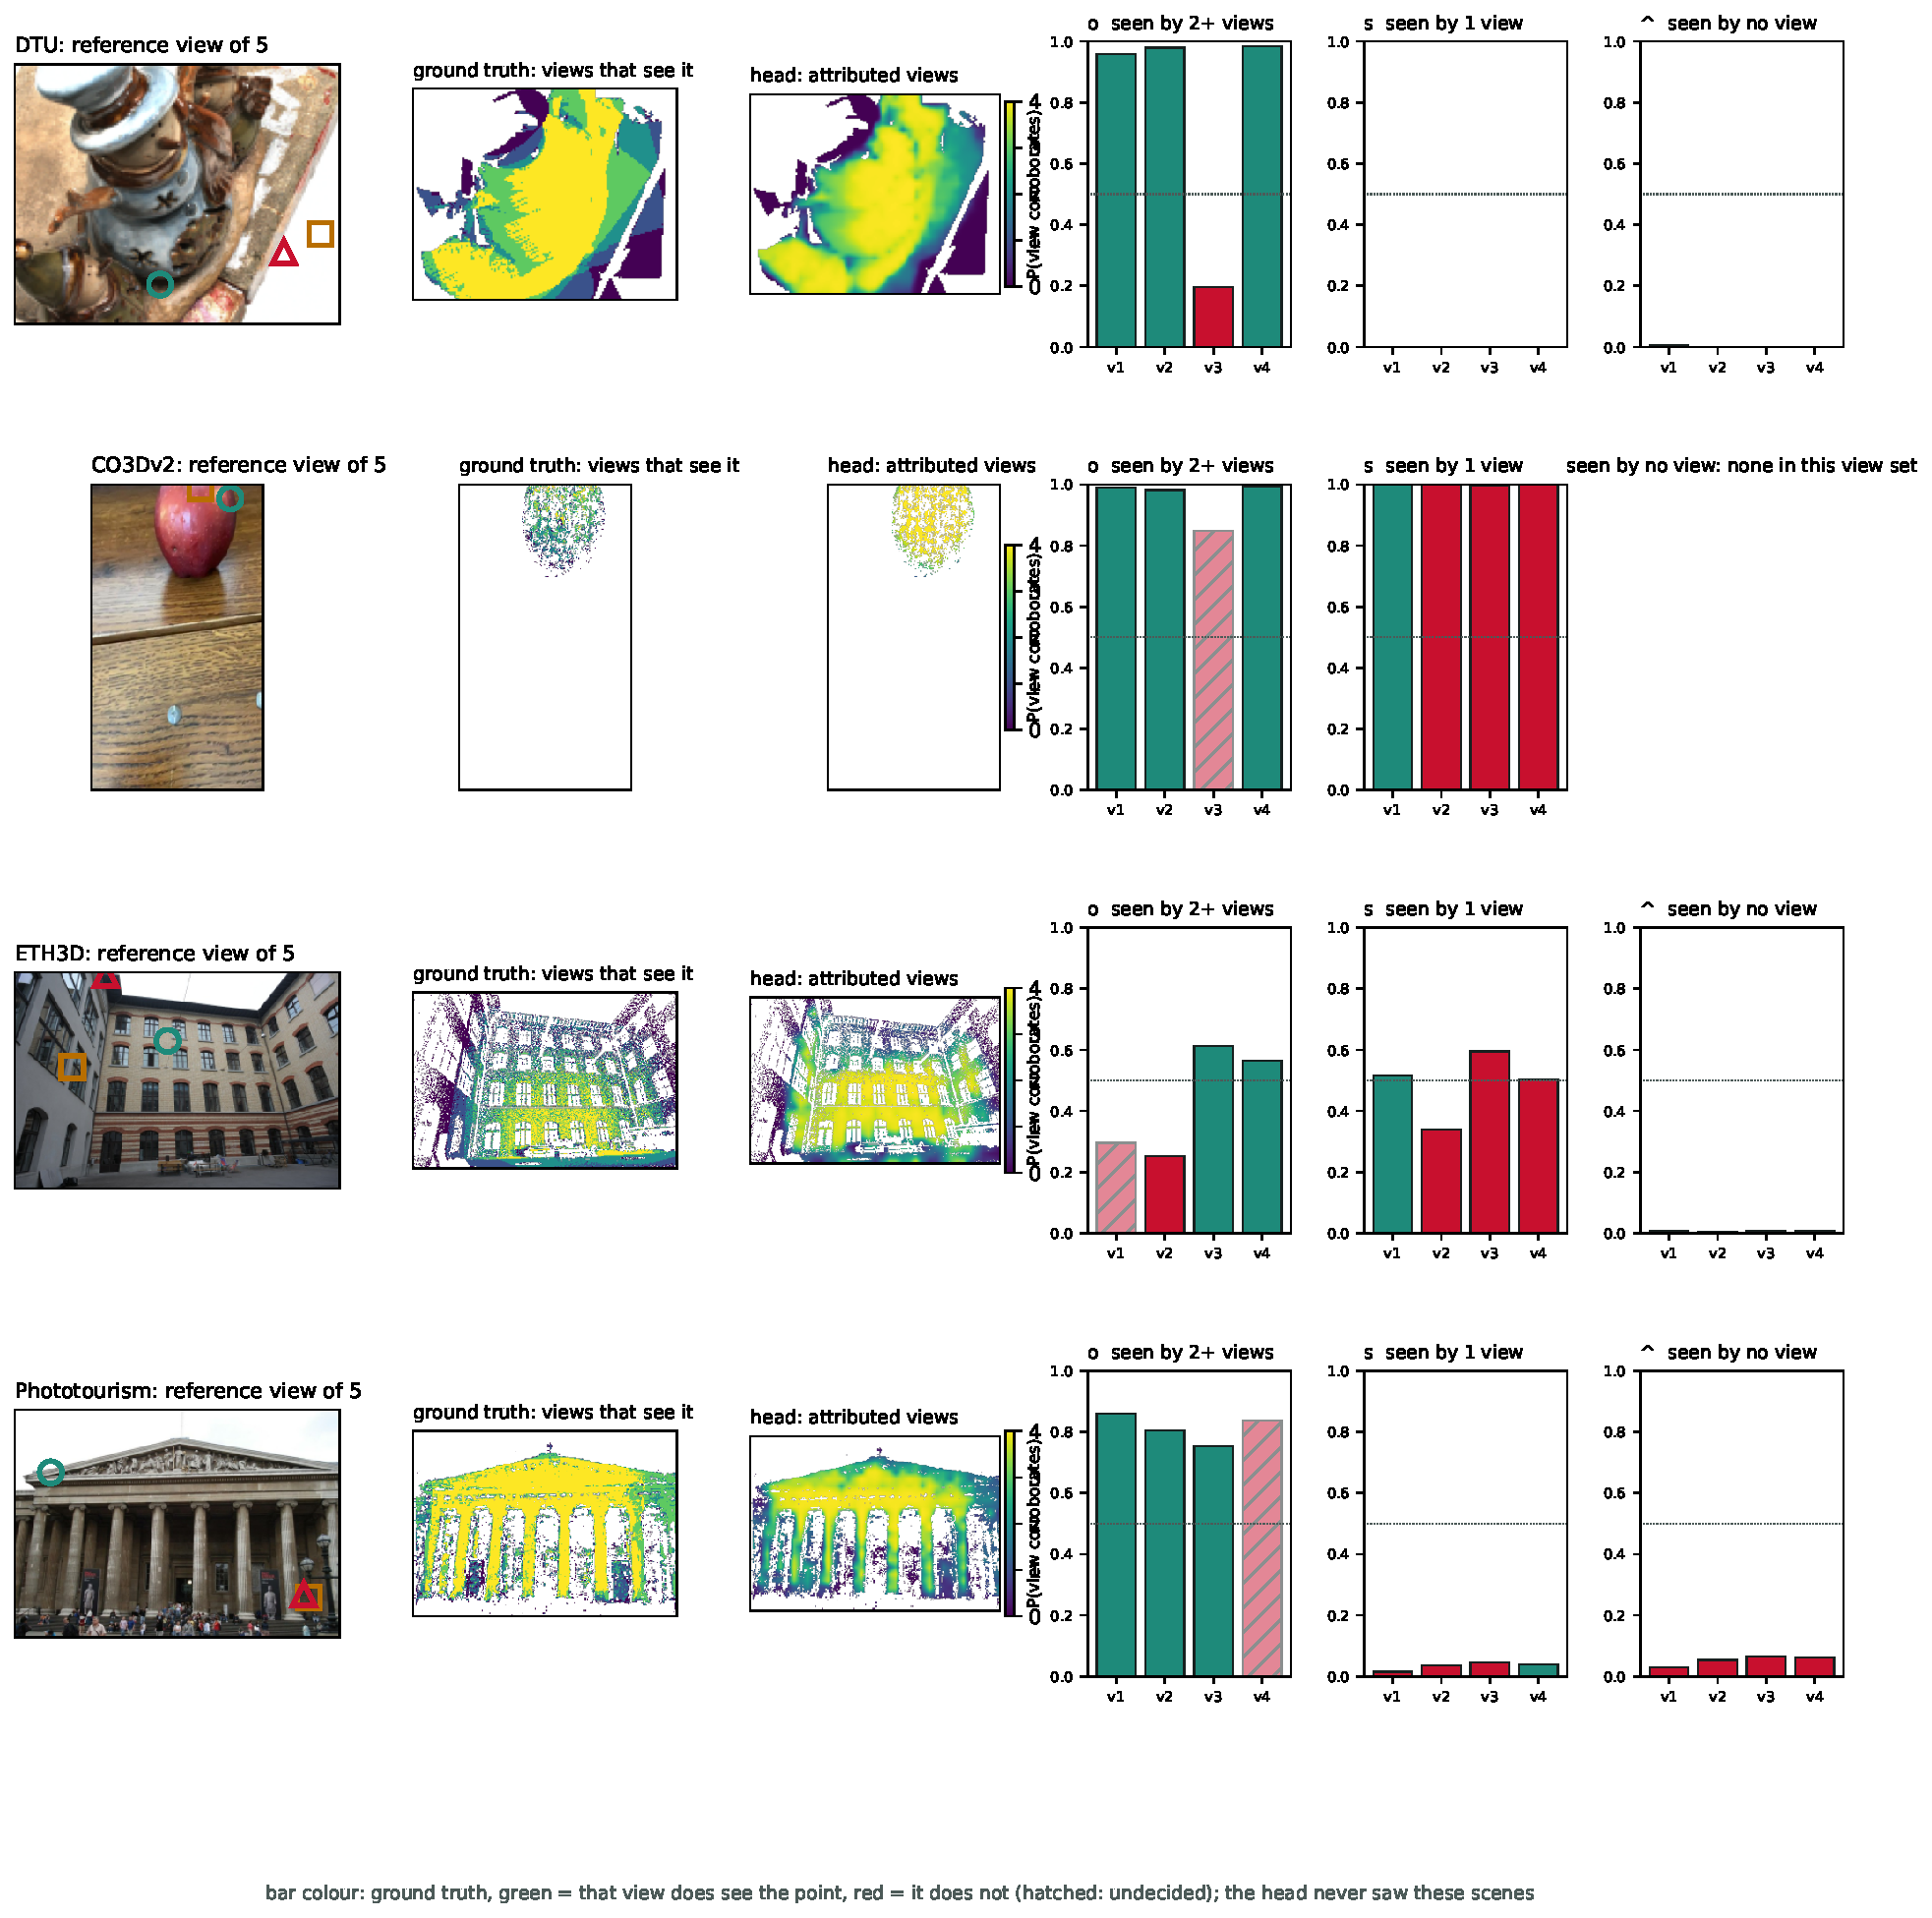
\includegraphics[width=\textwidth]{fig_prov_all}
\caption{\textbf{Which view saw it, one scene per dataset} (VGGT, label-free provenance head, five input views, scenes the head never saw). Per row: the reference view with three query pixels, the ground-truth number of other views that see each pixel, the number the head attributes, and the head's probability per other input view for each query (bar colour: ground truth). Run P10-prov.}
\label{fig:prov_all}
\end{figure}

\paragraph{Twenty views.}
With 20 clean DTU views, twice the most the heads saw in training (run P4-vis-ext), the visibility heads score \auroc{} 0.990 to 0.993 and the label-free heads 0.990 to 0.992, native confidence falls to 0.61 (VGGT) and 0.83 (Pi3X), reprojection consistency scores 0.93 and 0.89, and the per-image control rises to 0.94: with twenty views the few remaining single-view pixels sit at the frame edge, and the control reads the edge.

\paragraph{Pre-registered gates.}
The pass conditions were written into the run registry before the corresponding heads were trained, and the registry is versioned with the code. Gate 3 (true-visibility head; written 2026-11-06, before any visibility head was trained; the training kernels ran from commit \texttt{4132d11}): the head counts as detecting missing support when, pooled over 3, 5 and 10 views on DTU, (a) it beats native confidence on \auroc{} and \cur{} (paired sign-flip $p<0.05$), (b) it beats its per-image control on \auroc{} by at least 0.02 at $p<0.05$, and (c) both conditions hold on at least one dataset the head never saw (CO3Dv2 or ETH3D); if (b) fails, the single-view-support signal is reported as recoverable from per-image features and the method claim is dropped. Gate 4 (label-free head; written 2026-11-06 16:51 UTC, before any label-free head was trained, commit \texttt{c7e6919}): on DTU and on CO3Dv2, (a) and (b) as above against its own per-image control, and (c) within 0.03 \auroc{} of the ground-truth-trained head on DTU and ahead of reprojection consistency on CO3Dv2 at $p<0.05$ (its training signal is the reprojection test, so it has to generalise better than its teacher); if (a) or (b) fails the head is dropped, if only (c) fails it is reported as an ablation. Gate 5 (provenance head; written 2026-11-07 18:31 UTC, before any provenance head was trained, commit \texttt{f36fbd6}): the label-free provenance head replaces the conv head as the method of record when (a) its support score is within 0.02 \auroc{} of the conv head on every dataset and backbone, (b) its attribution beats the reprojection test read per view on prov-\auroc{} at $p<0.05$ on DTU and on at least two of CO3Dv2, ETH3D and the landmarks, for at least three backbones, and (c) its top-1 view sees the point for at least 90\% of the supported pixels on DTU; if (a) fails it is an attribution add-on, if (b) fails the attribution is reported as measured and the claim is reduced to reading per-view evidence at one forward, if (c) fails ``which view'' is not claimed. Outcome (run P10-prov, Table~\ref{tab:prov}): (a) holds on 15 of the 16 cells (Pi3X on CO3Dv2: $-0.025$), (b) fails (ahead of reprojection on DTU only, for three backbones), (c) holds (0.98 to 0.99); the conv head stays the method of record. Gate 6 (matched split; written 2026-11-08 06:05 UTC, commit \texttt{74aa0a3}, before any matched run): for each native model, (a) the leak survives the matched control when \cur$_m$'s interval excludes 0 and \auroc$_m<0.95$, (b) a model is patch-inflated when its original \auroc{} exceeds \auroc$_m$ by more than 0.10, in which case the matched numbers become its headline. Outcome: (a) holds for all five; (b) VGGT patch-inflated (share +0.389); Pi3 patch-inflated (share +0.427); Pi3X patch-inflated (share +0.344); MapAnything patch-inflated (share +0.237); DA3 patch-inflated (share +0.293). Gate 7 (matched heads; same registration): the per-image control must score at most 0.60 \auroc$_m$ on DTU (pipeline check), then the matched head must beat it by at least 0.10 ($p<0.05$), beat native confidence, reach 0.75 on the one-view low-parallax bucket, hold on CO3Dv2 without retraining, and its label-free variant must be within 0.03 of the ground-truth-placed one. Outcome: VGGT control 0.587, head 0.763, label-free 0.754; clauses a/b/c/e pass/pass/fail/pass; CO3Dv2 label-free head 0.681, control 0.575 (clause d); Pi3X control 0.591, head 0.730, label-free 0.693; clauses a/b/c/e pass/pass/fail/fail; CO3Dv2 label-free head 0.675, control 0.583 (clause d). Gate 8 (real occlusion against the 49-view scan; same registration): the share of predicted points on surfaces no input view observed is reported per backbone and view count; a detection claim needs that share to reach 0.5\% and the label-free head to beat native confidence at $p<0.05$. Outcome: share 1.1 to 1.3\% at 3 views, 0.5 to 0.8\% at 5, 0.2 to 0.4\% at 10 (VGGT, Pi3X); head against native on observed-versus-unobserved points, VGGT 0.81 / 0.90 / 0.92 against 0.80 / 0.80 / 0.78 ($p=0.29$, $<0.0001$, $<0.0001$), Pi3X 0.78 / 0.82 / 0.89 against 0.68 / 0.70 / 0.71 ($p\le0.0004$): the claim holds for Pi3X at 3 and 5 views and for VGGT at 5 views, not for VGGT at 3 views. The earlier Gate 2 (fill-trained head) had the clause ``head ahead of the control at $p<0.05$'' with no margin; it passed by the letter on differences of 0.0004 and 0.003 and the paper does not count it, which is why Gate 3 carries a margin.

\paragraph{Gaussian-splatting backbone (partial run).}
AnySplat (reference in the paper), a feed-forward 3D Gaussian-splatting model, was scored on the DTU configuration with its per-pixel Gaussian opacity as confidence (120 of 540 rows) and with the rendered accumulated alpha (450 of 540 rows), bf16 on one L4, run P3-gs. Pooled over blur and noise: opacity \auroc{} 0.583 / \cur{} 0.718, rendered alpha 0.632 / 0.745, \curerr{} 0.02 and 0.06; the noise fill drives the opacity below chance (0.36). The representation does not change the answer: a Gaussian the model places on an unseen surface is as opaque as one on an observed surface. The run stopped behind other jobs on the shared card and is reported as partial.

\paragraph{Run registry.} Every table cell maps to a run id (P1-full, P2-full, P2-stress, P2-co3d, P2-co3d-b, P3-pv-smoke, P2-smoke-b, P3-native, P3-reproj, P3-pv, P3-oia-dtu, P3-oia-abl, P3-oia-stress-*, P3-kaggle-vggt) whose CSV, configuration JSON and kernel log are released with the code, together with the dated log of every failed run and every correction.
